\documentclass[14pt, titlepage,fleqn]{extarticle}
\usepackage[T1,T2A]{fontenc}
\usepackage[utf8]{inputenc}

\usepackage{amsmath}
\usepackage[russian]{babel}

\usepackage{titlepage}
\usepackage[final]{pdfpages}
\usepackage{listings}
\usepackage{color}
\usepackage{graphicx}
\usepackage{float}
\usepackage{mathrsfs}
\usepackage{amsmath,amsfonts}

\usepackage{caption}

\newcommand{\Image}[2]{
	\begin{figure}[H]
		\center{\includegraphics[width = 0.4 \textwidth]{#1}}
		\caption{#2}
	\end{figure}
}

\definecolor{dkgreen}{rgb}{0,0.6,0}
\definecolor{gray}{rgb}{0.5,0.5,0.5}
\definecolor{mauve}{rgb}{0.58,0,0.82}

\lstset{frame=single,
	language=Python,
	aboveskip=3mm,
	belowskip=3mm,
	showstringspaces=false,
	columns=flexible,
	basicstyle={\small\ttfamily},
	numbers=none,
	numberstyle=\tiny\color{gray},
	keywordstyle=\color{blue},
	commentstyle=\color{dkgreen},
	stringstyle=\color{mauve},
	breaklines=true,
	breakatwhitespace=true,
	tabsize=3
}


\DeclareMathOperator{\Ci}{Ci}
\DeclareMathOperator{\Si}{Si}

\begin{document}
\selectlanguage{russian}

\fefutitlepage{Б9119--02.03.01сцт}{Панченко Н.К.}{17}{мая}{22}

\newpage

\tableofcontents
\clearpage
\section*{Введение}
\addcontentsline{toc}{section}{Введение}
Реализовать алгоритм построения интегрального преобразования Фу-
рье для произвольно-заданных функций одной переменной. 
\newpage









\section*{Постановка задачи}
\addcontentsline{toc}{section}{Постановка задачи}
Для реализации алгоритма потребуются следующие параметры:

\begin{itemize}
	\item $f(t)$ -- опредление функции,
	
	\item $a, b$ -- область интегрирования функции,
 
	\item $n_1$ -- количество разбиений области интегрирования (также мож-
	но использовать шаг $h_1$),	

	\item $n_2$ -- количество разбиений частотного диапазона (также можно
	использовать шаг $h_2$),

	\item $m$ -- максимальное значение частоты.
\end{itemize}

Задача сводится к построению спектрального разложения одно-
мерного сигнала $f(t)$ на частоты составляющих его волн.

Реализация проводится с помощью численных методов рассче-
та интегралов. Потребуется построить график функции $f(t)$, и ее
вещественные и комплексные спектральные разложения($\mathscr{F}_\Re\{f\}$ и $\mathscr{F}_\Im\{f\}$). Графики разложений строятся в диапазоне $\omega \in [0, m]$. Оси
графиков разложений представляют из себя по горизонтали - частотный диапазон, по вертикали - амплитуда.

Решение оформить в среде \LaTeX.
\newpage









\section*{Эксперимент}
\addcontentsline{toc}{section}{Эксперимент}
Рассмотрим функцию $f(t) = \sin t$ на диапазоне $[a, b] = [0, \pi]$, в остальном диапазоне полагая $f(t) = 0$. Для аналитического решения, функция примет вид: $f(t) = \sin t \cdot \Pi_{0,\pi}(t)$. Положим $\chi = 2\pi\omega$. Тогда преобразование Фурье примут вид:

\[\mathscr{F}_\Re\{\sin{t}\} = \int\limits_{-\infty}^{\infty} \sin{t} \cdot \Pi_{0,\pi}(t) \cdot \cos{\chi t}~dt = \int\limits_{0}^{\pi} \sin{t} \cos{\chi t} ~dt = \dfrac{\sin{\pi \chi}}{1 - \chi^2},\]

\[\mathscr{F}_\Im\{\sin{t}\} = \int\limits_{-\infty}^{\infty} \sin{t} \cdot \Pi_{0,\pi}(t) \cdot \sin{\chi t}~dt = \int\limits_{0}^{\pi} \sin{t} \sin{\chi t}  ~dt = \dfrac{\cos{\pi \chi + 1}}{1 - \chi^2}.\]  

В таком случае спектральный график в аналитической форме
будет иметь следующий вид:
\Image{graf.pdf}{Спектральный график волн синуса и косинуса (красный – ко-
синус, синий – синус)}
В результате реализации численного алгоритма, максимальное
значение частоты выберем $ m = 2$. Таким образом, численно найден-
ный спектральный график имеет вид:

\begin{figure}[H]
	\center{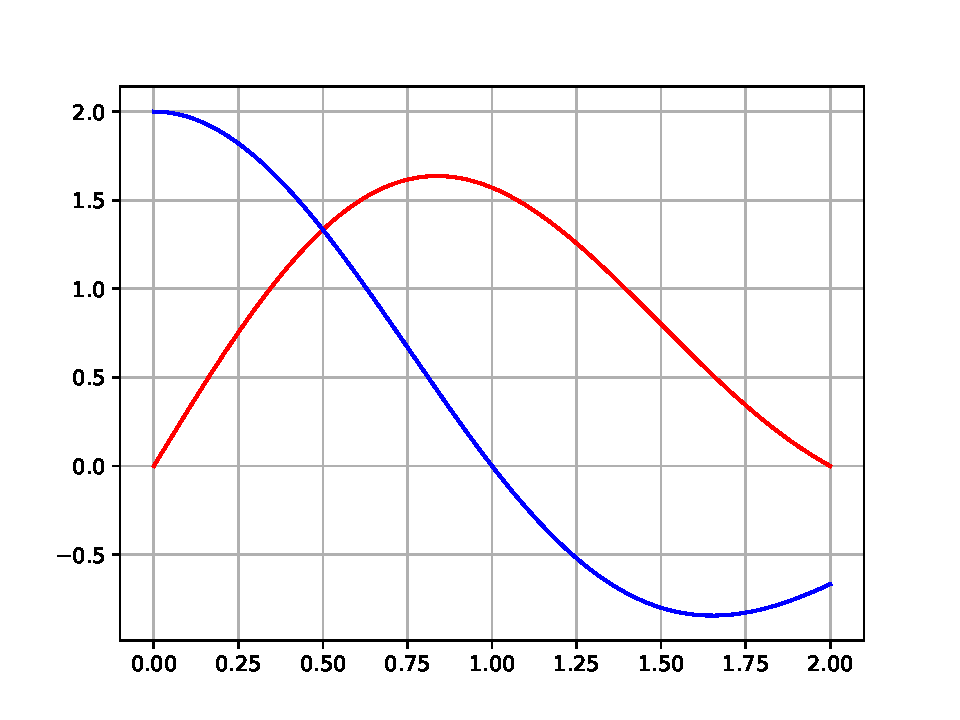
\includegraphics[width = 0.7\textwidth]{Figure_2.pdf}}
	\caption{Численно рассчитанный спектральный график волн синуса и
	косинуса (синий – косинус, оранжевый – синус)}
\end{figure}
\newpage










\section*{Решение}
\addcontentsline{toc}{section}{Решение}
Рассмотрим функцию $f(t) = \dfrac{t}{1 - 4t^2}$ на диапазоне $[a, b] = \left[0, \dfrac{1}{4}\right]$, в остальном диапазоне полагая $f(t) = 0$. Для аналитического решения, функция примет вид: $f(t) = \dfrac{t}{1 - 4t^2} \cdot \Pi_{0,\frac{1}{4}}(t)$. Положим $\chi = 2\pi\omega$. Тогда преобразование Фурье примут вид:

\[\mathscr{F}_\Re\left\{\dfrac{t}{1 - 4t^2}\right\} = \int\limits_{-\infty}^{\infty}  \dfrac{t}{1 - 4t^2} \cdot \Pi_{0, \frac{1}{4}}(t) \cdot \cos{\chi t}~dt = \int\limits_{0}^{ \frac{1}{4}}  \dfrac{t}{1 - 4t^2}  \cos{\chi t} ~dt = \]

\[=- \dfrac{(-1)^\omega \Ci{\left(\frac{3\pi \omega}{2}\right)}}{8} + \dfrac{(-1)^\omega \Ci{(\pi \omega)}}{8} - \dfrac{(-1)^\omega \Ci{\left(-\frac{\pi \omega}{2}\right)}}{8} + \dfrac{(-1)^\omega \Ci{(- \pi \omega)}}{8}.\]

\[\mathscr{F}_\Im\left\{\dfrac{t}{1 - 4t^2}\right\} = \int\limits_{-\infty}^{\infty}  \dfrac{t}{1 - 4t^2} \cdot \Pi_{0,\frac{1}{4}}(t) \cdot \sin{\chi t}~dt = \int\limits_{0}^{ \frac{1}{4}}  \dfrac{t}{1 - 4t^2}  \sin{\chi t} ~dt = \]

\[=- \dfrac{(-1)^\omega i\Si{\left(\frac{3\pi \omega}{2}\right)}}{8} + \dfrac{(-1)^\omega i\Si{(\pi \omega)}}{8} - \dfrac{(-1)^\omega i\Si{\left(-\frac{\pi \omega}{2}\right)}}{8} + \dfrac{(-1)^\omega i\Si{(- \pi \omega)}}{8}.\]

% В таком случае спектральный график в аналитической форме
% будет иметь следующий вид:
\begin{figure}[H]
	\center{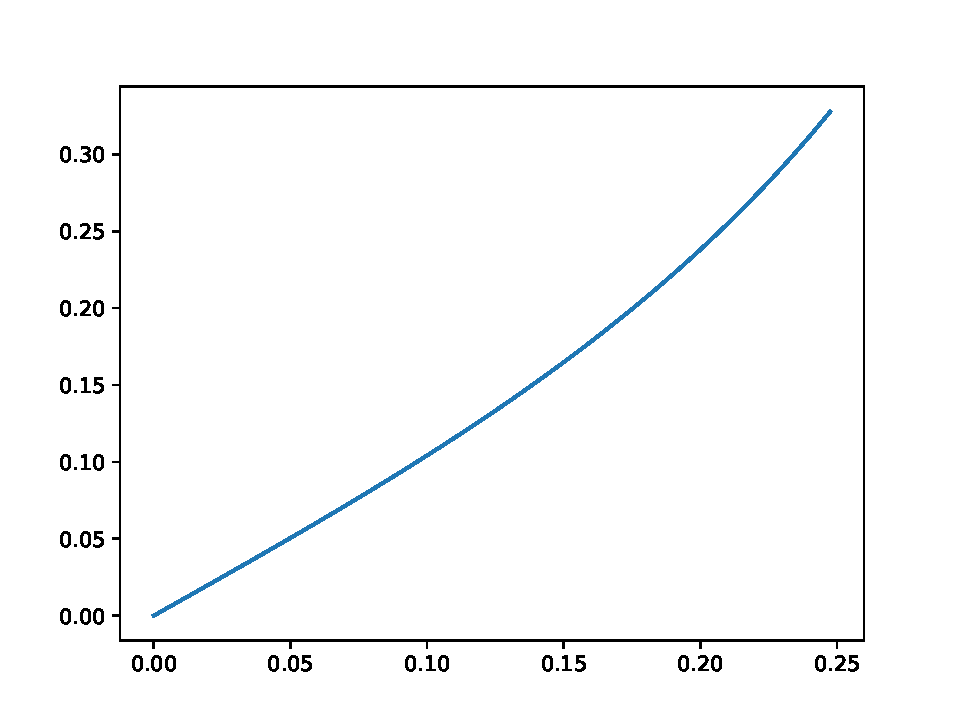
\includegraphics[width = 0.7\textwidth]{f1.pdf}}
	\caption{График функции}
\end{figure}


В результате реализации численного алгоритма, максимальное
значение частоты выберем $m = 2$. Таким образом, численно найден-
ный спектральный график имеет вид:

\begin{figure}[H]
	\center{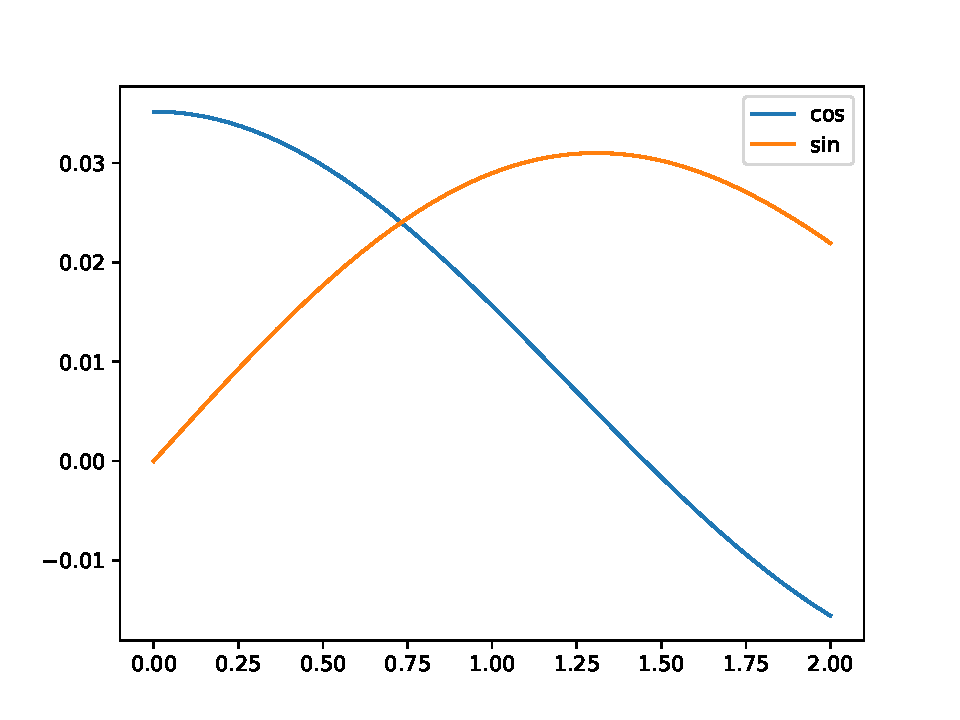
\includegraphics[width = 0.7\textwidth]{g2.pdf}}
	\caption{Спектральный график волн синуса и косинуса}
\end{figure}
\newpage









\section*{Код}
\addcontentsline{toc}{section}{Код}

\begin{lstlisting}
def f(t):
    return t / (1 - 4 * t**2)

def intelCos(t, w):
    return cos(2 * pi * w * t)


def intelSin(t, w):
    return sin(2 * pi * w * t)


def intel(f, x, func, w):
    return (sum([f(i) * func(i, w) * (x[-1] - x[0]) / len(x) for i in x]))

a = 0
b = 1/4
h1 = 200
h2 = 1000
m = 2
x = [(i / h1) * (b - a) + a for i in range(h1)]
y = [f(i) for i in x]
W = [i / h2 * m for i in range(h2)]
integ = [[integ(f, x, intelCos, i), integ(f, x, intelSin, i)] for i in W]

\end{lstlisting}
\newpage









\section*{Заключение}
\addcontentsline{toc}{section}{Заключение}
Во время выполнения данной лабораторной работы была решена поставленная задача и оформелена в \LaTeX.
\end{document}